A variety of physical processes in the photospheres and chromospheres of stars 
can lead to time-correlated radial velocity signals that are cohesively 
referred as \emph{stellar jitter}. Especially in radial velocity, stellar jitter 
signals are the bane of us observers because the jitter signals can mask and 
in certain instances even mimic the planetary signals that we are searching for. \\

Depending on the exact physical process, these 
signals can have widely differing timescales and manifestations in 
spectroscopic, photometric, and polarimetry observations. In general jitter 
signals are also wavelength dependent unlike Doppler variations induced by 
planetary companions. Ancillary timeseries to radial velocity measurements 
derived from any of the aforementioned observations can therefore be used to 
disentangle radial velocity jitter from Doppler signals. A detailed list 
of examples of such timeseries is presented in Sect.~\ref{sect:diagnostics}. 
Firstly, I describe the various 
sources of stellar jitter, their associated timescales, and approximate 
amplitudes in radial velocity. 

\section{Sources of Stellar Jitter} \label{sect:jitter}
\subsection{Flares}
Magnetically active stars can undergo energetic flares or coronal mass 
ejections originating from the stellar atmosphere. The exact flare physics 
in M-dwarfs is still uncertain but clearly requires strong magnetic fields 
which can be sustained by turbulent convective motions and rotation 
\parencite{browning08}. Flare events result in sudden increases in brightness 
followed by an exponential brightness decay over a \textbf{few minutes}. The rapid 
brightness increase from flares have been observed across the electromagnetic 
spectrum (X-ray: \cite{osten10}; UV: \cite{hawley07}; optical: 
\cite{kowalski09}; radio: \cite{osten08}). Fig.~\ref{fig:flare} depicts the 
characteristic light curve profile as well as the 
increase in line strengths and equivalent 
widths for the UT 2009 October 27 flare on the mid-M flare star, EV Lac. \\

\begin{figure}
\centering
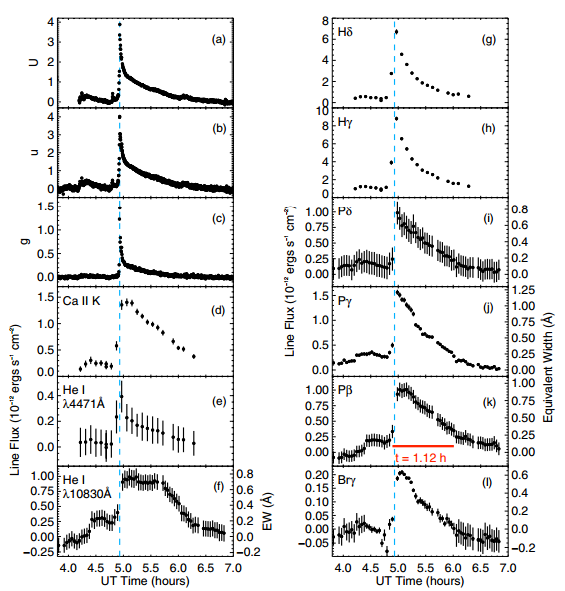
\includegraphics[scale=.6]{figures/flarelines.png}
\caption{\emph{Panels a,b,c}: the $U,u$, and $g$ band light curves during an 
observed flare on the mid-M flare star, EV Lac. The remaining panels similarly 
depict the variation to the line flux and line equivalent width 
for numerous optical and near-IR lines. 
\parencite[Image credit:][]{schmidt12} \label{fig:flare}}
\end{figure}

Flares are easily identified in stellar spectra as certain emission lines of 
hydrogen, helium, and/or ionized metals, 
in both the optical and near-IR (e.g. H$\alpha$, H$\delta$; 
\cite{reiners09}; P$\beta$, P$\gamma$, P$\delta$, Br$\gamma$; 
\cite{schmidt12}) are 
excited beyond the quiescent state and decay shortly afterwards. 
The corresponding radial velocity spike is large; 
\textbf{tens of m s$^{\mathbf{-1}}$}. Because radial velocity 
measurements affected by flares can be easily identified by the characteristic 
line intensity spike over short timescales, such radial velocity 
measurements are commonly removed from the analysis.

\subsection{Stellar Oscillations}
Most of the information in this subsection comes from \cite{christensen14}. \\

Small scale adiabatic perturbations to the internal mechanical structure of 
stars can give rise to oscillation modes. If not damped, these oscillations 
can propagate through the stellar interior before rebounding at the surface 
of the star thus creating an observable radial velocity pulse of a 
\textbf{few m s$^{\mathbf{-1}}$} 
on a timescale of a \textbf{few to tens of minutes} \parencite{bedding01}. 
Fig.~\ref{fig:rvpulsation} shows the differential Doppler shift at the 
stellar surface as a result of the complex distortion of the surface and 
the corresponding spectral line profile distortion to help visualize the 
way in which the observed radial velocity of the star is affected by (in this 
case) non-radial pulsation modes. \emph{This phenomenon is predominantly 
observed in Sun-like and post-MS stars}. Due to the short timescale of 
pulsation variations in radial velocity measurements of pulsating stars, the 
jitter is mitigated through the use of sufficiently long exposure times 
\parencite{lovis05, dumusque11}. \\

\begin{figure}
\centering
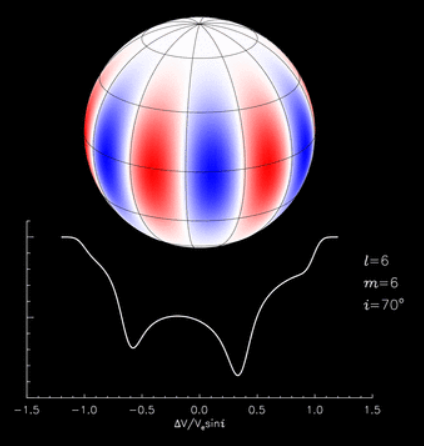
\includegraphics[scale=.5]{figures/nonradial_pulsationsmall.png}
\caption{\emph{Blue} and \emph{red} regions depict the distortion of the
stellar surface by non-radial pulsation modes towards and away from the observer
respectively. The corresponding spectral line distortion is shown in the
\emph{lower panel}. \parencite[Image credit:][]{kochukhov16} \label{fig:rvpulsation}}
\end{figure}

Stellar oscillation modes typically 
manifest themselves as either acoustic pressure waves (p-modes) or gravity 
waves (g-modes). The former exist due to the restoring force arising from 
fluid pressure and propagate at the local adiabatic sound speed 

\begin{equation}
c_s = \sqrt{\frac{\Gamma_1 k_B T}{\mu}},
\end{equation}

\noindent for an ideal gas where $\Gamma_1$ is the adiabatic exponent ($5/3$ 
for a monoatomic gas), $k_B$ is the Boltzmann 
constant, $T$ is the local temperature, and $\mu$ is the mean molecular weight 
of the gas. The sound waves become trapped between the stellar surface and an 
inner turning point $r_t$ located where the characteristic acoustic frequency 

\begin{equation}
S_l^2 = \frac{l (l+1) c^2}{r^2} 
\end{equation}

\noindent equals the angular frequency of the oscillation mode satisfying 
the dispersion relation of the wave: $\omega^2 = c^2 |\mathbf{k}|^2$ where 
$|\mathbf{k}|=2\pi/\lambda$ and $\lambda$ is the wave's wavelength. 
Here $l$ is the degree of the spherical 
harmonic solution to the mechanically perturbed differential equations of 
stellar structure. Fig.~\ref{fig:astero} shows the propagation of 
two acoustic waves with varying degree $l$ near the stellar surface. In the 
Sun, modes with $l \gtrsim 40$ are trapped within the Sun's convection zone. \\

\begin{figure}
\centering
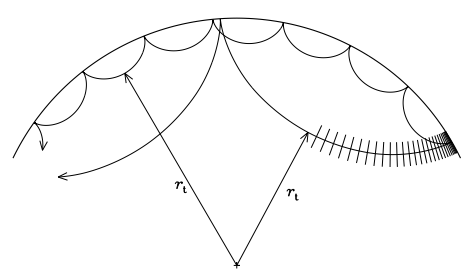
\includegraphics[scale=.5]{figures/asteroseismology.png}
\caption{Propagation of p-mode standing waves with penetration to large depths 
($l=30$) and shallow depths ($l=100$). Orthogonal lines represent the wave 
fronts at equal time intervals along the $l=30$ mode's path. 
\parencite[Image credit:][]{christensen14} \label{fig:astero}}
\end{figure}

The latter wave (g-modes) 
experiences a restoring force due to gravity which acts against 
buoyancy forces across horizontal surfaces with the buoyancy, or 
Brunt-V\"{a}is\"{a}l\"{a} frequency 
 
\begin{equation}
N^2 = g \left( \frac{1}{\Gamma_1} \frac{\mathrm{d} \ln{P}}{\mathrm{d}r} - 
\frac{\mathrm{d} \ln{\rho}}{\mathrm{d}r} \right),
\end{equation}

\noindent where $g,P$ and $\rho$ are the local gravitational acceleration, 
pressure, and density respectively. \\

Fig.~\ref{fig:propagation} shows the regions in the Sun in which the mechanical 
oscillations are driven as p or g-modes. The p-mode curve is plotted for a 
mode with $l=1$. In the over-lapping region the oscillations are referred to as 
mixed modes. \\

\begin{figure}
\centering
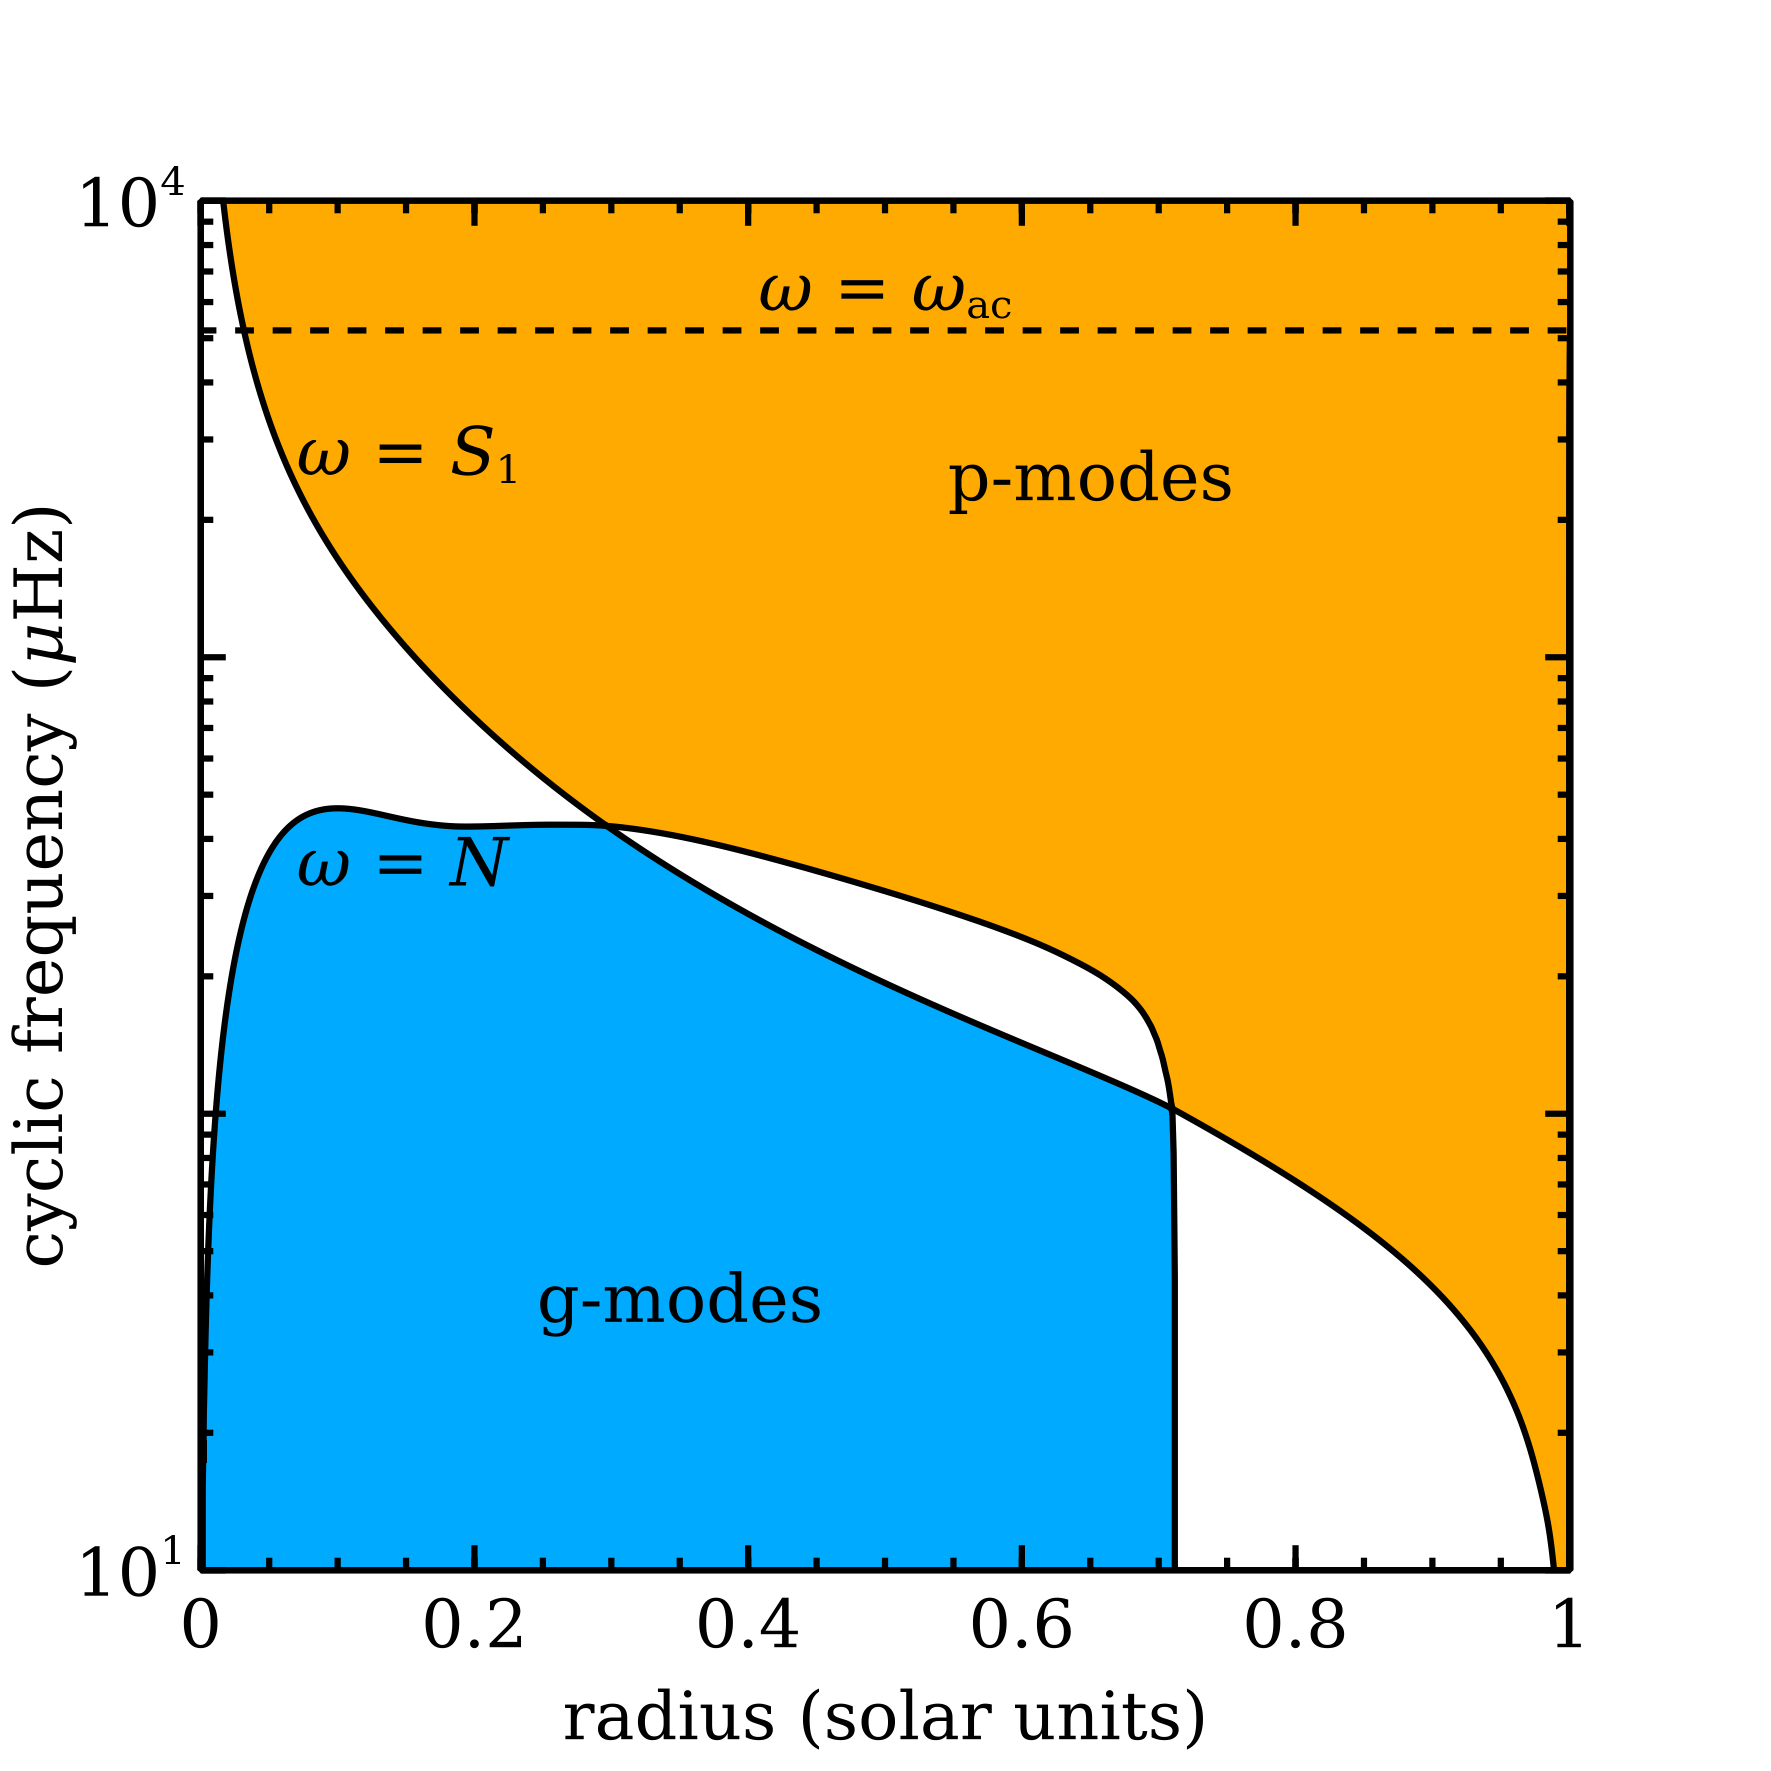
\includegraphics[scale=.5]{figures/Propagation_diagram.png}
\caption{Depiction of where in the solar model mechanical oscillations are 
characteristically p-modes, g-modes, or a mixture of the two. The acoustic-cutoff 
is shown with the \emph{dotted horizontal line} and represents the maximum frequency 
at which resonant modes remain `trapped' within the solar interior.  
\parencite[Image credit:][]{christensen96} \label{fig:propagation}}
\end{figure}

\subsection{Granulation}
Stars with outer convection zones such as the Sun and M-dwarfs will exhibit granulation 
at their surface. The granulation pattern is the result 
of convection cells penetrating the surface; hot fluid parcels rising to the surface before 
cooling and descending back into the stellar interior (see Fig.~\ref{fig:granulation}). \\

\begin{figure}
\centering
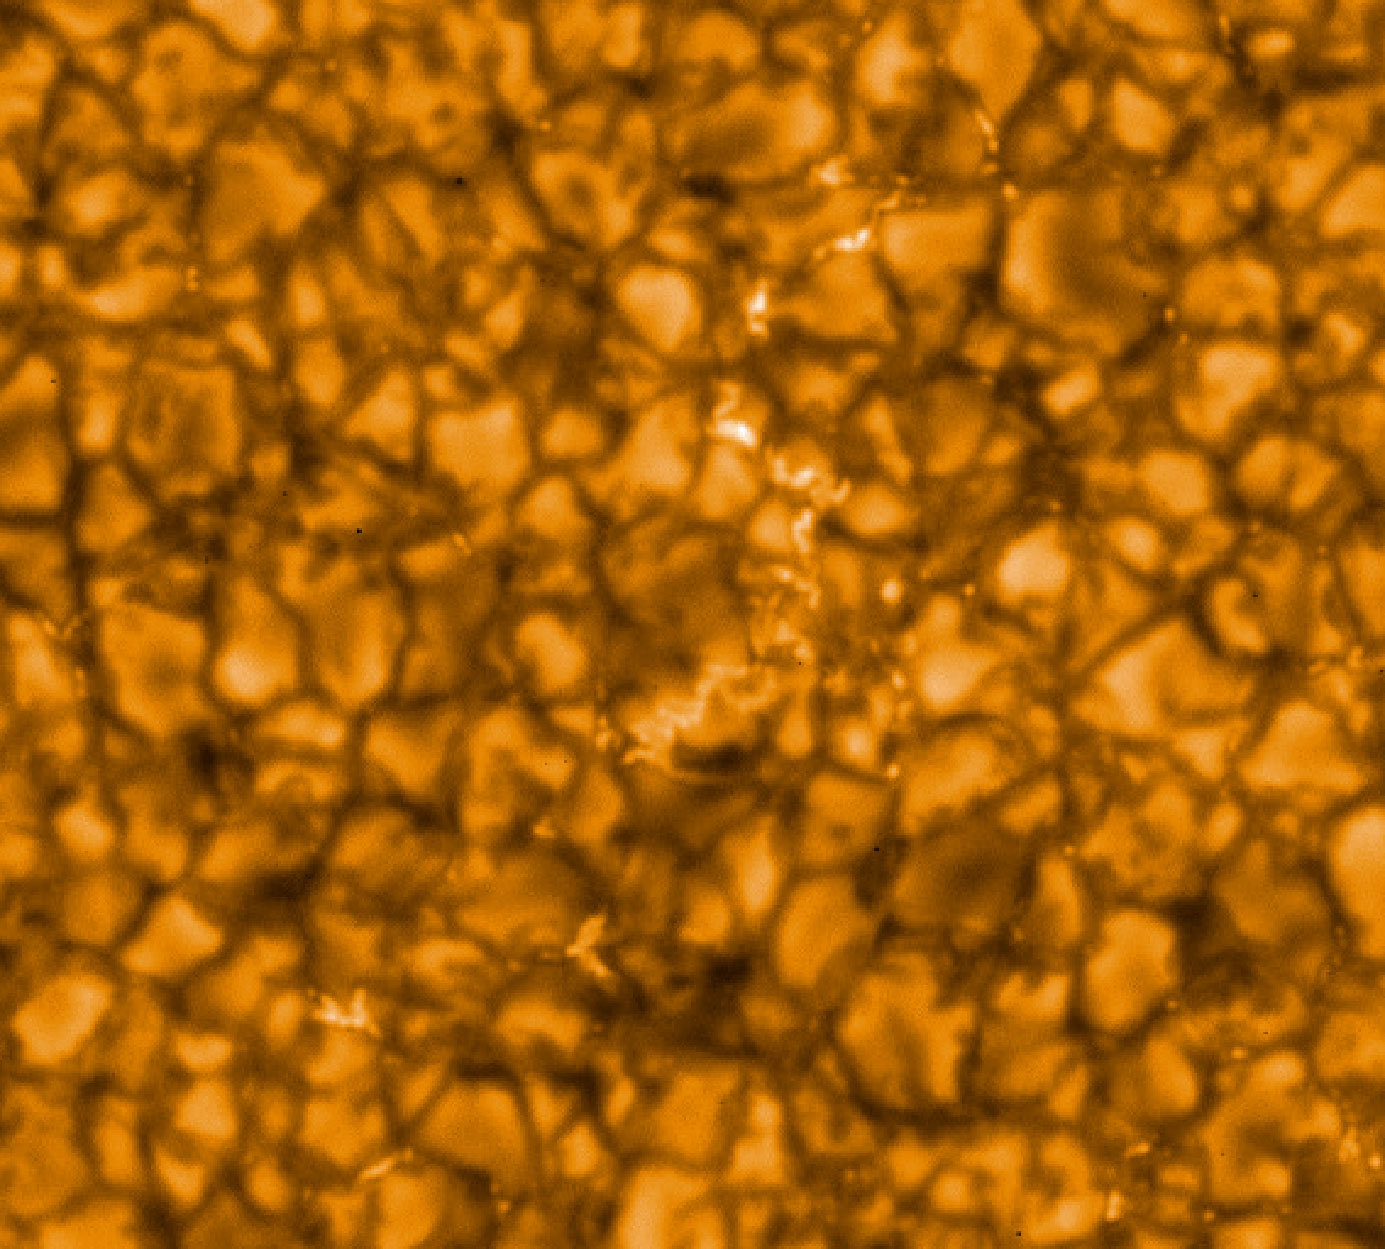
\includegraphics[scale=.2]{figures/solargranulation.jpg}
\caption{An image of a patch of the solar surface taken with NASA's Hinode Optical 
Telescope. The bright regions are the result of rising hot fluid parcels whereas the cooler, 
``intergranular lanes'' reveal where the gas has cooled and descends back into the solar 
interior. (Image credit: Hinode JAXA/NASA/PPARC) \label{fig:granulation}}
\end{figure}

Patches of hot rising fluid are brighter than the regions of cold descending fluid. 
Furthermore, the relative fractional coverage of a star by rising fluid parcels is 
in general greater than that of descending ones as evidenced in Fig.~\ref{fig:granulation}. 
Because the rising parcels have their radial velocity component pointed towards a distant 
observer, photons emitted from these hot parcels at the photospheric boundary are blueshifted 
whereas the cold, ``intergranular lanes'' are redshifted. The domination of the stellar 
surface area by hot parcels results in a granulated star having a net \emph{convective 
blueshift}. \\

The short lifetimes of \emph{typical} granules ($\mathbf{\sim 10}$ \textbf{minutes}; 
\cite{hall08}) means that brightness variability of the surface varies on a similar timescale. 
Such variations have been measured using high cadence photometry \parencite[e.g.][]{gilliland11}.
The corresponding radial velocity jitter is dependent on the relative velocity of convective 
cells across the stellar surface. Noting that the relative sizes of granules varies over time, so 
too does the resulting radial velocity component whose \emph{net} effect (hot and cold regions partially 
cancel each other) is a \textbf{few m s$^{\mathbf{-1}}$} \parencite{lindegren03}. This level of radial 
velocity jitter has been observed on both the Sun \parencite{kuhn83} and on $\alpha$ Cen A 
\parencite{kjeldsen99}. \\

In addition to \emph{typical} granules with sizes of a few hundred km \parencite{hall08}, there 
also exist classes of larger and longer-lived granules. These include `mesogranules' with lifetimes of 
tens of minutes \parencite{roudier98} up to `supergranules' which can persist for up to a day 
\parencite{delmoro04}. \\

Similarly to the radial velocity observing strategy designed to mitigate the effect of short-timescale 
stellar oscillations, the noise induced by typical granulation has been sufficiently beat-down with multiple 
observations per night \parencite{lovis05, dumusque11}.

\subsection{Spots, Plages, and Faculae (...oh my!)}
Like the Sun, the photospheres of active late-type stars are often littered with dark star spots 
and/or hot faculae or plages in the chromosphere. In the Sun these structures have long been known to 
be associated with strong local magnetic fields as evidenced by the observed Zeeman splitting 
(see Sect.~\ref{sect:zeeman}) of lines emitted from these so-called \emph{active regions} 
\parencite{hale08}. 

\subsubsection{Active regions: timescales}
The jitter from active regions is 
\textbf{modulated by the projected stellar rotation velocity} \vsini{} or alternatively, the stellar rotation 
period $P_{\mathrm{rot}}$. The stellar rotation period can be measured for active stars with non-zero 
inclination ($i_s \ne 0^{\circ}$) from the periodicity in its photometric variability. 
Because active regions are associated with magnetic activity and stellar 
magnetic fields require rotation in order to be sustained over long timescales, rapidly rotating 
late-type stars tend to be magnetically active; they exhibit strong jitter signals from active regions. 
Fig.~\ref{fig:activity} demonstrates that the fraction of M-dwarfs which are active \parencite{west15} 
decreases as the main-sequence stars spin-down over time via magnetized braking from stellar winds 
\parencite{skumanich72}. \emph{Therefore the stellar rotation period can be used as a first-order 
indicator of an M-dwarf's activity level}. Fig.~\ref{fig:rotation} depicts the rotation period 
distribution of M-dwarfs in the solar neighbourhood \parencite{newton16a} and in the Kepler 
field up to just $P_{\mathrm{rot}} < 70$ days \parencite{mcquillan13a}. 
Two distinct populations exist, namely a rapidly 
rotating population ($P_{\mathrm{rot}} \lesssim 3$ days) and a slowly rotating population 
($P_{\mathrm{rot}} \gtrsim 50$ days). It has been proposed that the two populations 
have a distinct range of ages. That is that 
the slow rotators belong to an older stellar population based on their galactic 
kinematics \parencite{irwin11} resulting from magnetic-braking over time. 
Indeed a robust relation exists for GK and early M-dwarfs between stellar 
mass, age, and rotation \parencite[gyrochronology;][]{barnes03}. \\

\begin{figure}
\centering
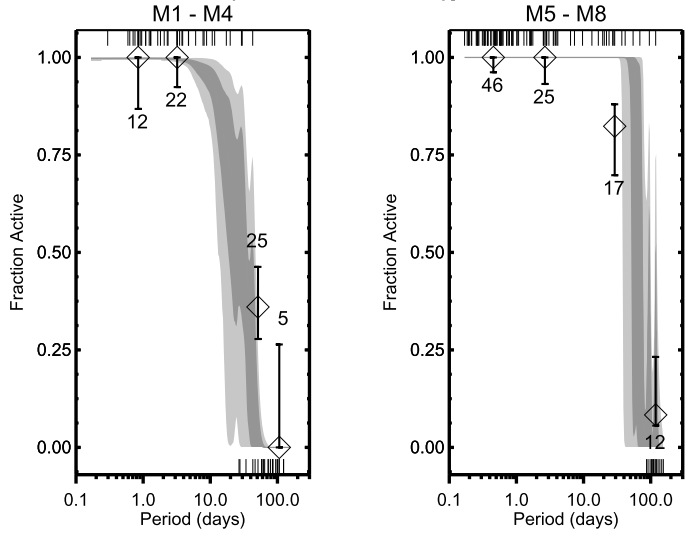
\includegraphics[scale=.5]{figures/mdwarfactivity.png}
\caption{The fraction of active M-dwarfs, as probed by the presence of strong H$\alpha$ 
emission, as a function of stellar rotation period for `early-to-mid' (\emph{left panel}) and 
`mid-to-late' (\emph{right panel}) M-dwarfs. 
\parencite[Image credit:][]{west15} \label{fig:activity}}
\end{figure}

\begin{figure}
\centering
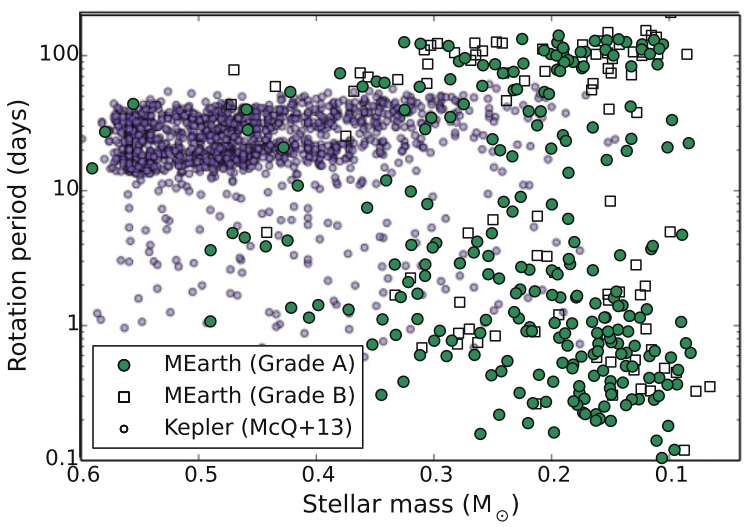
\includegraphics[scale=.5]{figures/mdwarfrotation.png}
\caption{Rotation period vs. stellar mass for solar neighbourhood (MEarth) and Kepler field 
M-dwarfs. Periods of the Kepler stars are intentionally capped at $P_{\mathrm{rot}}=70$ days. 
\parencite[Image credit:][]{newton16a} \label{fig:rotation}}
\end{figure}

Another important point regarding active regions is that their lifetimes are comparable 
to the stellar rotation timescale. This means that the associated stellar jitter can vary 
between rotation cycles. As seen in Fig.~\ref{fig:rotation}, 
the lifetimes can be from days to months 
\parencite{schrijver02}. Active region 
lifetimes are primarily determined by their sizes \parencite{berdyugina05} as they 
diffuse into the photosphere; larger volume/surface ratios results in longer lifetimes 
\parencite{robinson82, petrovay97}. 

\subsubsection{Active regions: spots} \label{sect:spots}
The re-connection of magnetic field loops with the surface inhibit the convective energy 
transport and results in star spots having cooler temperatures relative to the surrounding 
unspotted photosphere. The temperature differences are typically 
$\sim 500-2000$ K \parencite{schrijver02, berdyugina05}. Without the temperature  
anomaly from star spots (or any other active region), 
the stellar disk would be homogeneous. In this case the opposing 
blue and redshifted stellar limbs would exactly cancel. 
However if that symmetry is broken by the 
presence of star spots then the disk-integrated spectral line profile will be asymmetric 
as shown in Fig.~\ref{fig:starspot} thus resulting in an anomalous radial velocity 
signal proportional to the stellar rotation \vsini{.} This is commonly known as the 
flux effect and is at the level of $\sim 1$ \mps{} for the Sun with its $\sim 24$ day 
equatorial rotation period \parencite{lagrange11}. The flux effect can be \textbf{more 
than an order of magnitude larger} for more rapidly rotating stars. \\

\begin{figure}
\centering
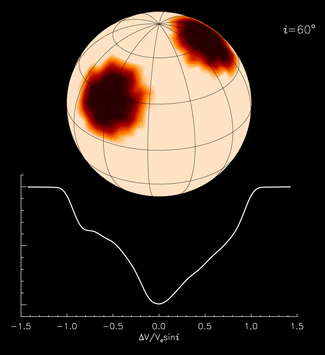
\includegraphics[scale=.5]{figures/starspot.png}
\caption{An example of a spotted stellar photosphere. The cool spots disrupt the symmetry of the 
disk-integrated spectral line profile according to the temperature difference between the spot and 
unspotted photosphere at its position on the stellar disk. 
\parencite[Image credit:][]{kochukhov16} \label{fig:starspot}}
\end{figure}

Star spot properties such as their fractional coverage of the stellar surface and the 
brightness contrast are degenerate in photometric observations of 
brightness variations. A technique known as \emph{Doppler imaging} \parencite{vogt83} 
may however be able to disentangle 
these effects and measure the size distribution of star spots. 
Doppler imaging works by tracking the spectral line profile distortion over time. 
Spectroscopic observations, which as we saw in Fig.~\ref{fig:starspot} 
are sensitive to the presence 
of active regions on the visible stellar disk. These distortions observed 
over the rotation cycle of a 
star can be used to derive the locations and sizes of star spots. These observations 
can then be used to reconstruct brightness maps such as those shown in 
Fig.~\ref{fig:brightnessmap} for two T-Tauri stars. Because the strength of line 
distortions is amplified by rotation, these observations are best suited to rapid 
rotators with long-lived star spots which can be mapped over multiple rotation cycles. \\

\begin{figure}
\centering
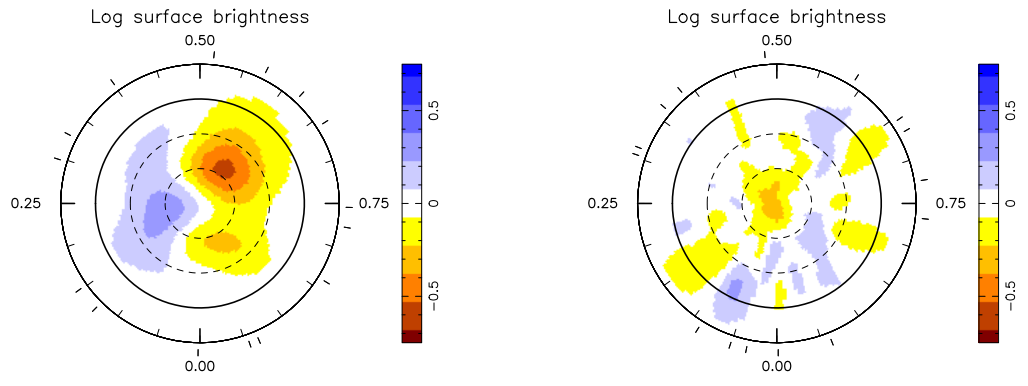
\includegraphics[scale=.4]{figures/surfacemap.png}
\caption{Relative surface brightness maps of the T-Tauri stars V819 (\emph{left}) and V830 
(\emph{right}) from Doppler imaging. 
The logarithmic brightness is measured relative to the quiet photosphere. 
The surface maps are projected onto 2D polar coordinates from one pole down to a latitude 
of $-30^{\circ}$. \parencite[Image credit:][]{donati15} \label{fig:brightnessmap}}
\end{figure}

\subsubsection{Active regions: faculae and plages} \label{sect:plages}
In addition to cool spots in the photosphere, 
faculae are hot bright regions that occupy the intergranular lanes and also surround  
cool star spots \parencite{thomas08}. However they may also form their own networks 
independent of spots. On the Sun their lifetimes can range from a few hours up to months 
for the larger networks of faculae \parencite{hirayama78}. Faculae tend to dominate 
a star's population of active regions if the star is slowly rotating whereas rapid rotators 
tend to be dominated by spots \parencite{lockwood07}. In stars exhibiting significant 
coverage by faculae, the temperature difference 
between the hot faculae and the remaining photosphere is only $\sim 100$ K \parencite{thomas08} 
so the corresponding photometric signal is small. However the strong magnetic fields in the 
faculae regions strongly suppress the convective blueshift thus causing a significant 
spectroscopic signature even in the absence of an equivalent photometric signal 
\parencite{meunier10}. \\

Stellar chromospheres can also harbour corresponding bright regions 
known as plages. These regions 
map well to the presence of spots and faculae in the underlying photosphere 
\parencite{hall08}. Hot plages in the hot chromosphere give rise to various emission 
lines such as H$\alpha$ and \caii{} lines which are often used 
to measure stellar activity \parencite{cincunegui07}. \\

Both plages and faculae have a similar flux effect to that of spots (see Sect.~\ref{sect:spots}). 
The only difference being that the observed flux in the Doppler shifted stellar emission lines is 
greater than in the quiet photosphere rather than being a deficit because of the positive temperature 
difference. Therefore the resulting jitter signal can again \textbf{range from tens of cm s$^{-1}$ 
to many tens of \mps{} if the star is undergoing rapid rotation.}

\subsection{Magnetic Cycles}
The Sun undergoes a magnetic cycle with an 11 year period as measured by the fractional 
coverage/number of sunspots and faculae \parencite{hathaway10}. At solar maximum, the 
peak in magnetic activity over the solar cycle, the Sun i) experiences strong prominences 
and coronal mass ejections and ii) has large number of visible active regions on its surface  
which tend to settle near the equator as evidenced in the famous `butterfly diagram' 
\parencite[see Fig.~\ref{fig:butterfly};][]{maunder04}.  \\

\begin{figure}
\centering
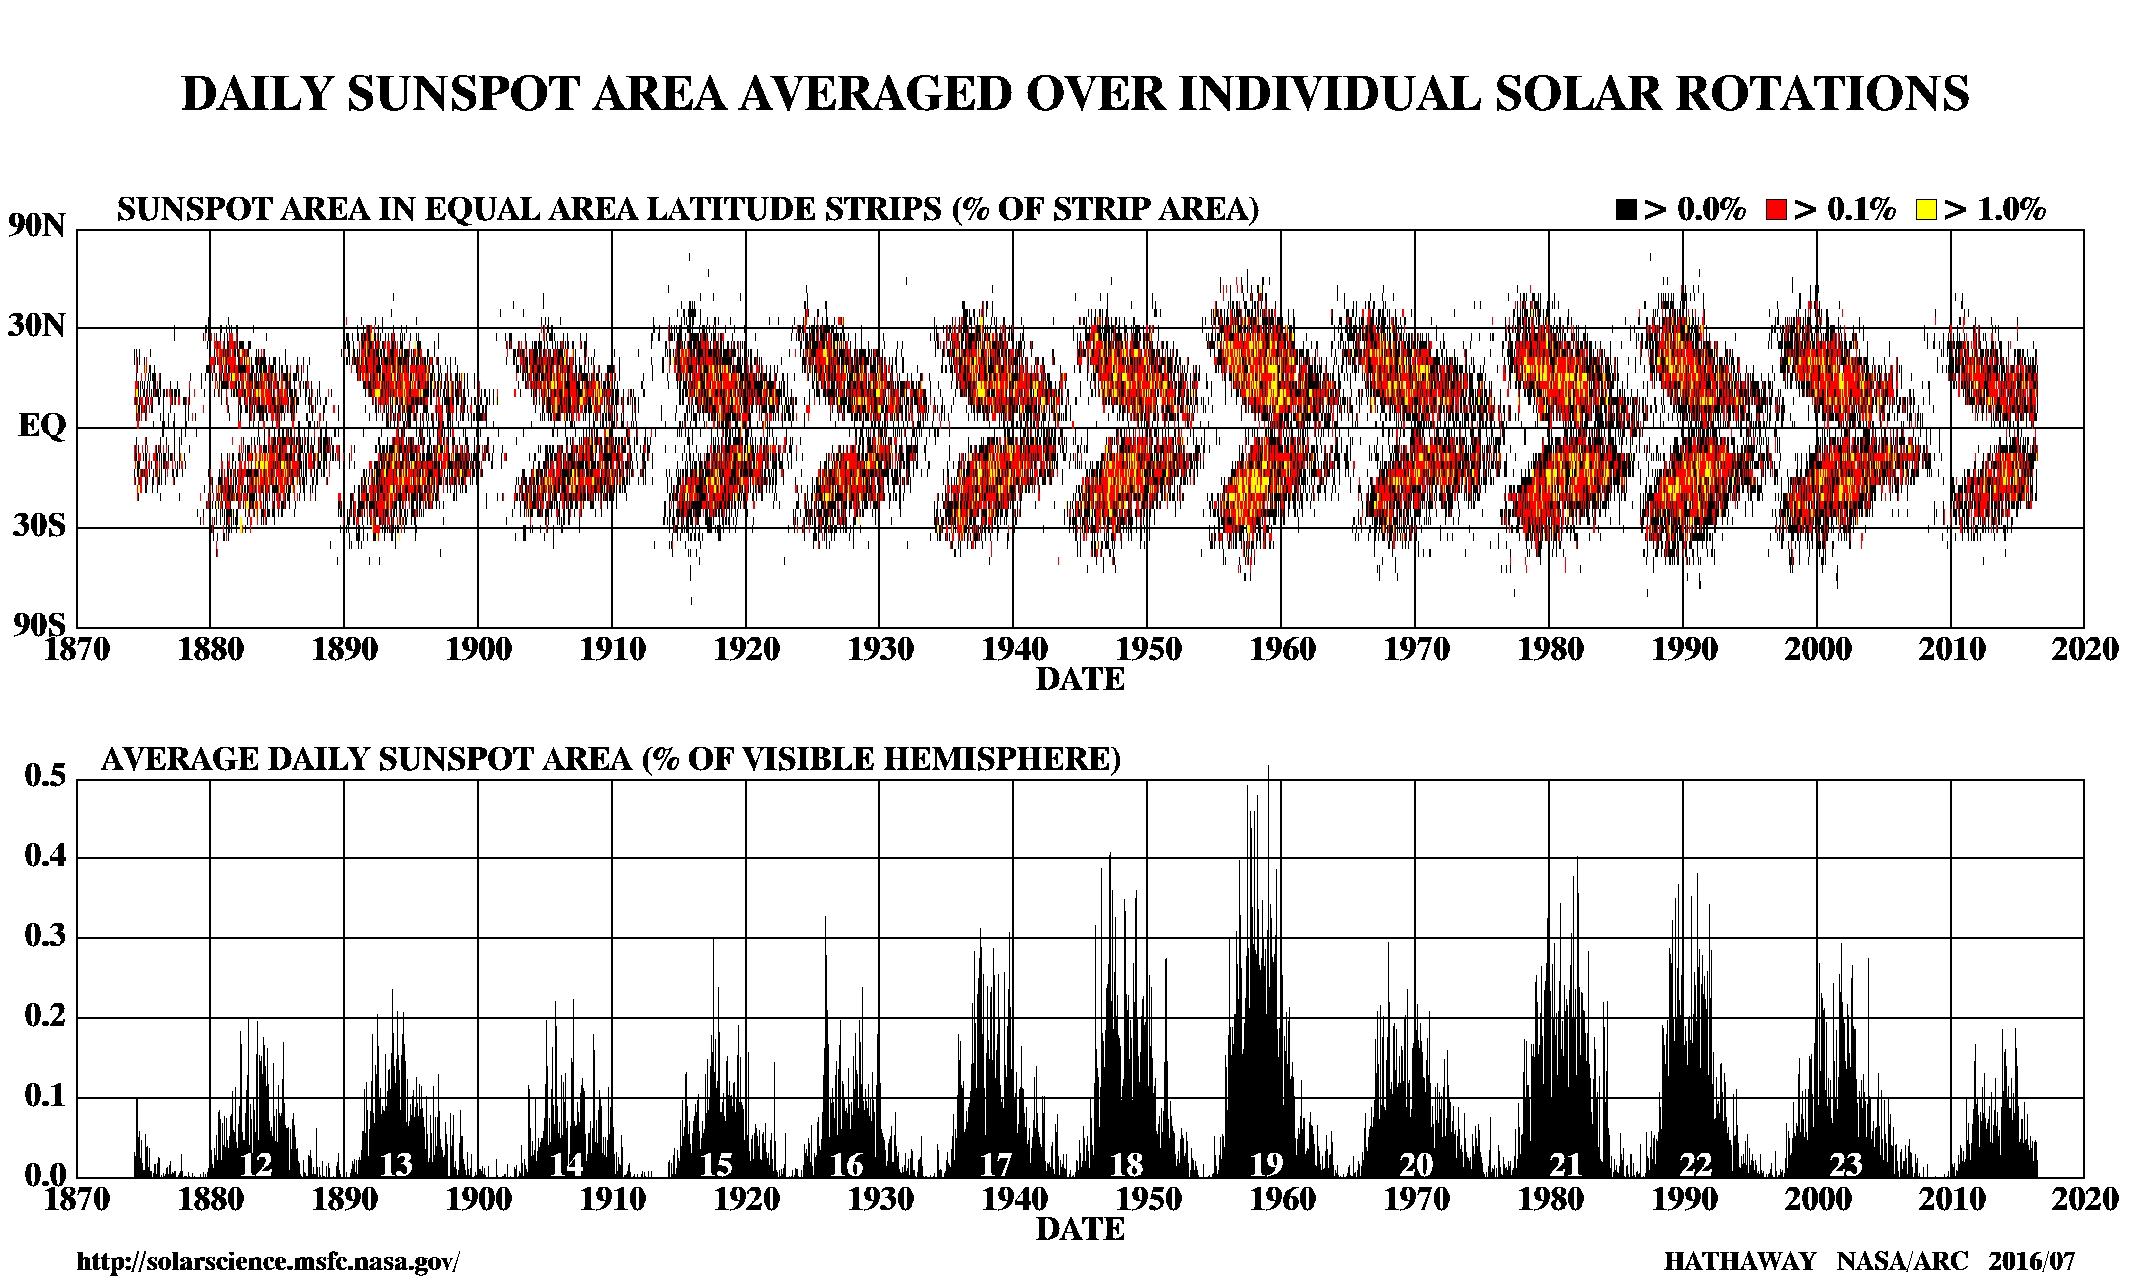
\includegraphics[scale=.2]{figures/bfly.png}
\caption{Timeseries of the coverage of the solar surface by sun spots in terms of the 
number of spots (\emph{top}) and fractional spot area (\emph{bottom}). The plot demonstrates 
the periodicity of the solar cycle; period $\sim 11$ years. 
\parencite[Image credit:][]{hathaway10} \label{fig:butterfly}}
\end{figure}

Long-term magnetic activity cycles have been observed with long-baseline spectroscopic 
monitoring initiatives. From solar observations, the flux in the \caii{} 
H and K lines were known to correlate with the number of Sun spots and therefore 
the level of activity \parencite{leighton59}. Numerous results from similar 
surveys have 
demonstrated that the majority of Sun-like stars do exhibit magnetic activity cycles 
with a range of periods from $\mathbf{\sim 7-30}$ \textbf{years} 
\parencite{duncan91, lockwood97, balinunas98}. \\

As it pertains to radial velocity searches for exoplanets, full activity cycles have yet 
to be observed and characterized. Subsections of the cyclic trends have been seen in  
certain mature radial velocity surveys \parencite[e.g.][]{lovis11} to be correlated with 
the $\log{R'_{\mathrm{HK}}}$ activity indicator (see Sect.~\ref{sect:indicator}). 
A common tactic is to use a timeseries of $\log{R'_{\mathrm{HK}}}$ and a linear relation to 
model the radial velocity variation from the indicator \parencite{dumusque12}. The radial 
velocity signal can be up to \textbf{tens of m s}$^{\mathbf{-1}}$. Luckily, when searching for 
planets with orbital timescales much less than the period of its star's magnetic cycle, the 
corresponding jitter is not of much concern. However when searching for distant giant planets 
in lengthy surveys, such as the 
upcoming \spirou{} Legacy Survey (see Sect.~\ref{sect:survey}), the long-term effects from 
magnetic activity cycles will need to be considered and modelled ideally using a spectral 
activity indicator like $\log{R'_{\mathrm{HK}}}$ but in the near-IR. \\

A summary of the approximate timescales and radial velocity signal amplitudes associated with 
each of the aforementioned sources of stellar jitter is given in Table~\ref{table:jitter}.

\newgeometry{margin=1cm}
\begin{landscape}
\begin{table*}
\caption{Summary of Radial Velocity Stellar Jitter}
\label{table:jitter}
\begin{tabular}{cccl}
  \hline
  \hline
  \textbf{Jitter Source} & \textbf{Timescale} & \textbf{Signal Amplitude} & \textbf{Notes} \\
  \hline
  Flares & a few minutes & tens of \mps{} & Has distinct photometric and spectroscopic signatures. \\ 
  &&&Observations during a flaring event should be excluded from \\
  &&&planet searches. \\
  \hline
  Oscillations & tens of minutes & few \mps{} & Can be mitigated with sufficiently long exposure times \\
  &&&or multiple observations per night. \\
  \hline
  Granulation & tens of minutes & few \mps{} & See oscillations.  \\
  \hline
  Active Regions & stellar rotation period & tens of cm s$^{-1} \to$ tens of \mps{} & See Fig.~\ref{fig:rotation} for the distribution of M-dwarf $P_{\mathrm{rot}}$. \\
  \hline
  Magnetic Cycles & $\sim  7-30$ years & tens of \mps{} & Is only important when searching for \\
  &&&long period planets.
  \end{tabular}
\end{table*}

\end{landscape}
\restoregeometry

\section{Activity Indicators} \label{sect:diagnostics}
A number of photometric, spectroscopic, and polarmetric indicators of stellar jitter are 
discussed below. 
Each of these signatures are unaffected by the gravitational influence of companions. We can 
therefore use any or all of these indicators to inform our model of stellar jitter in order 
to disentangle it from any underlying planetary signals. 

\subsection{Photometry}
Active regions, which give rise to a subset of radial velocity jitter processes, have a 
corresponding photometric signal due to the temperature difference between the active 
region and quiet stellar photosphere. High cadence photometry can then be used to monitor 
the motion of active regions across the stellar photosphere and be used to measure the 
stellar rotation period. Of course this only works if the stellar spin-axis is misaligned 
with the line-of-sight. Fig.~\ref{fig:lcgp} shows an example of a CoRoT light curve of the 
active\footnote{From photometry, CoRoT-7 has $>5$ times the spot coverage of the Sun 
\parencite{queloz09}.}, super-Earth hosting CoRoT-7 from \cite{haywood14}. The light curve 
is fit with a quasi-periodic Gaussian process (see Sect.~\ref{sect:gpformalism}). As we 
shall see in Sect.~\ref{sect:ffprime}, the smooth light curve model can be used to model the 
radial velocity jitter corresponding to the active regions causing the star's photometric 
variability as it rotates. \\

\begin{figure}
\centering
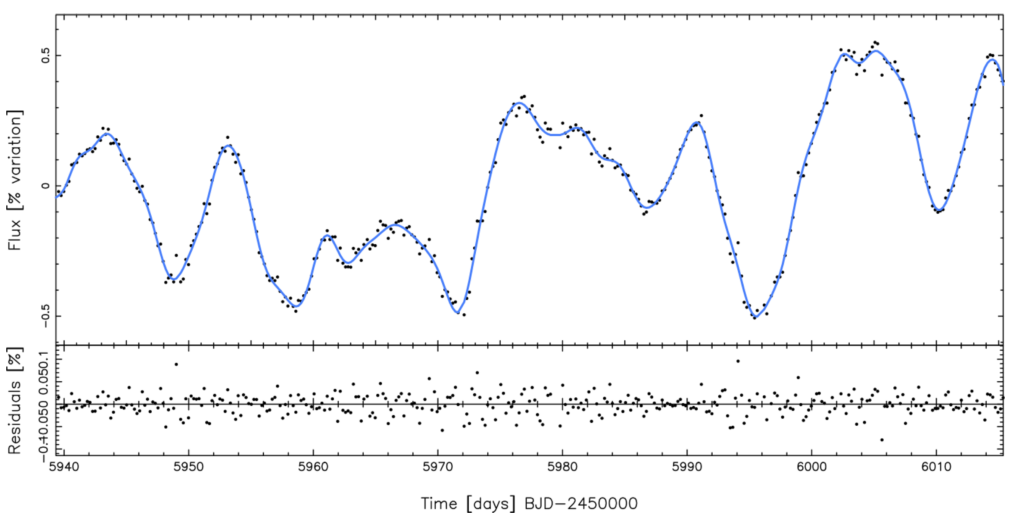
\includegraphics[scale=.4]{figures/lcgp.png}
\caption{\emph{Top panel}: the light curve of CoRoT-7 with a quasi-periodic Gaussian process 
fit to the data. \emph{Bottom panel}: residuals of the fit. \parencite[Image credit:][]{haywood14} 
\label{fig:lcgp}}
\end{figure}

\subsection{$R'_\mathrm{HK}$ Line Indicator} \label{sect:indicator}
As mentioned in Sect.~\ref{sect:plages}, emission from the cores of the singly ionized Ca 
H and K lines trace chromospheric activity. 
%Typically stellar photosphere is assumed to be 
%in local thermodynamic equilibrium (LTE) such that the source function equals the Planck 
%function at the local electron temperature. As one travels up from the photosphere the plasma 
%becomes optically thin and no longer in LTE 
\cite{thomas57} argued that in a Sun-like chromosphere the source of ionized metals such as 
\caii{} is dominated by collisional de-excitations rather than a 
radiative process. These lines are sensitive to the local electron temperature which varies 
within hot plages thus making the lines sensitive to the presence of such active regions 
\parencite{hall08}. The corresponding observable is called the $R'_{\mathrm{HK}}$ index and 
represents the emission in the chromospheric H and K line cores relative to the bolometric 
luminosity:

\begin{equation}
R'_{\mathrm{HK}} = \frac{\Psi_{\mathrm{H}} + \Psi_{\mathrm{K}}}{\sigma T_{\mathrm{eff}}^4},
\label{eq:rhk}
\end{equation}

\noindent where $\Psi_{\mathrm{H}}$ and $\Psi_{\mathrm{K}}$ are the fluxes in the cores of the 
H and K lines (3933.7 \& 3968.5 \AA) respectively, 
$\sigma$ is the Stefan-Boltzmann constant, and $T_{\mathrm{eff}}$ is the stellar effective 
temperature \parencite{martinez10}. The $R'_{\mathrm{HK}}$ is often expressed as $\log{R'_{\mathrm{HK}}}$. 
Although each of the H and K lines are at optical rest wavelengths, a near-IR 
spectral activity indicator defined similarly to Eq.~\ref{eq:rhk} may be useful for radial 
velocity surveys conducted with near-IR spectrographs such as \spirou{.}


\subsection{CCF: Full Width at Half Maximum} \label{sect:fwhm}
As we saw in Fig.~\ref{fig:starspot}, the temperature contrast between an active region 
(a cool spot in this example) breaks the symmetry of the disk-integrated spectral line profile 
or the CCF (see Sect.~\ref{sect:spectrograph}) of the entire observed stellar spectrum. Initially, 
the CCF is rotationally broadened by an amount which depends on the projected stellar 
rotation rate \vsini{} and pressure broadened thermal motions in the stellar photosphere. On top 
of these effects to the full width at half maximum (FWHM) of the CCF, the presence of active 
regions can also broaden the CCF depending on the active region's size, location, and contrast. 
Constructing timeseries of the CCF FWHM contemporaneously with radial velocity 
measurements, thus provides a 
means of monitoring the activity-related signals. Indeed the FWHM has been used in a number of 
observational studies \parencite[e.g.][]{queloz09, hatzes10}.

\subsection{CCF: Bisector Inverse Slope} \label{sect:bis}
An complementary activity indicator derived from the observed CCF is a measure of the line 
profile's 
asymmetry. The so-called bisector inverse slope (BIS) is commonly computed as the difference in 
the location of the bisector in the first 10-40\% of the CCF depth and the location of the 
bisector in ranging from 60-90\% of the CCF depth \parencite{dumusque14}. By this definition 
a quiet photosphere will have BIS = 0 \mps{} as the CCF is just Gaussian and therefore symmetric. \\

However recall that granulation produces a net convective blueshift meaning that the blue wing 
(negative velocity) of the disk-integrated CCF has more flux than the red wing. The resulting 
CCF therefore has a slightly positive BIS (see Fig.~\ref{fig:bis}). 
Recall that the presence of active regions 
suppresses the convective blueshift effect thus altering the measured BIS. The apparent correlation 
between the presence of active regions and the BIS again allows one to use a BIS timeseries to 
monitor the activity-related signal as has been done in observational studies 
\parencite[e.g.][]{queloz01}. \\

\begin{figure}
\centering
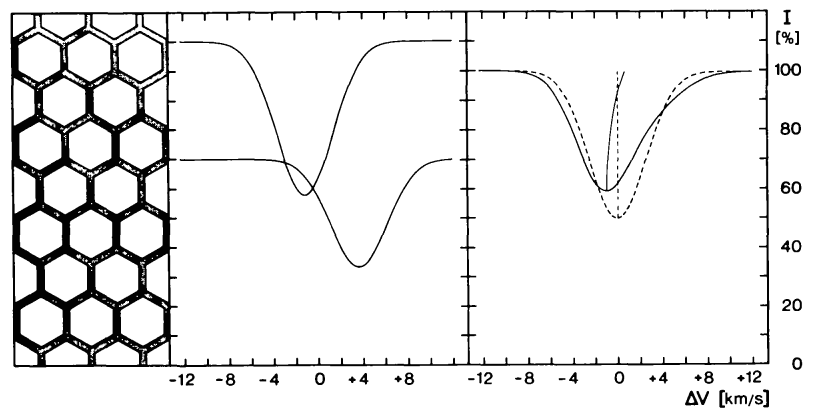
\includegraphics[scale=.4]{figures/bis.png}
\caption{\emph{Left}: an illustration of surface granulation with 75\% of the surface area 
being covered by rising granules and the remaining area belonging to the descending intergranular 
lanes. \emph{Middle}: idealized spectral CCFs for the granular regions (negative velocity; top) and 
intergranular lanes (positive velocity; bottom). \emph{Right}: the resulting disk-integrated 
CCF (average over the surface; \emph{solid curve}) compared to the undisturbed CCF (\emph{dashed 
curve}). \parencite[Image credit:][]{dravins81} \label{fig:bis}}
\end{figure}

\subsection{Multi-wavelength Radial Velocities}
Because the radial velocity jitter arising from active regions depends on the temperature contrast 
between the active region and the quiet photosphere, the resulting jitter amplitude is wavelength 
dependent. This is especially true in late-type stars as 
the brightness contrast decreases from the visible towards 
the near-IR \parencite{hebrard14}. Observationally, the radial velocity jitter from active regions 
is seen to be 
approximately a factor of four less in the near-IR than in the visible in low-mass and young 
T-Tauri stars \parencite[e.g.][]{martin06, huelamo08, prato08, mahmud11}. This is favourable for 
exoplanet searches with a near-IR instruments such as \spirou{.} However the apparent reduction in 
stellar jitter towards longer wavelengths is countered by the increased jitter from Zeeman 
broadening at near-IR wavelengths (see Sect.~\ref{sect:zeeman}) in rapidly rotating stars. Therefore 
it is not absolutely true that the jitter from active regions will necessarily 
decrease at near-IR wavelengths. \\

Unlike the stellar jitter, Doppler signals induced by the presence of planetary companions are 
achromatic. We can therefore write the observed radial velocities calculated at a central wavelength 
$\lambda$ as 

\begin{equation}
\mathrm{RV}_{\lambda}^{\mathrm{obs}}(t) = \sum_{i=1}^{N} \mathrm{K}_i(t) + 
\mathrm{RV}_{\lambda}^{\mathrm{jitter}}(t), \label{eq:rvtot}
\end{equation}

\noindent where RV$_{\lambda}^{\mathrm{jitter}}$ is the wavelength dependent intrinsic stellar jitter and 
the $N$ keplarian models K$_i$ (K$_i=v(t)$; see Eq.~\ref{eq:rv}) remain unaffected by changes in 
$\lambda$\footnote{Actually $\lambda$ should instead be written as a range of wavelengths instead of 
a single value because of the non-zero width of the spectral bands.}. 
Therefore if two radial velocity timeseries at two different wavelengths 
$\lambda_1$ and $\lambda_2$ can be obtained with a sufficiently large SNR, 
the difference between the two timeseries will not contain any keplarian component:

\begin{equation}
\mathrm{RV}_{\lambda_1}^{\mathrm{obs}}(t) - \mathrm{RV}_{\lambda_2}^{\mathrm{obs}}(t) = 
\mathrm{RV}_{\lambda_1}^{\mathrm{jitter}}(t) - \mathrm{RV}_{\lambda_2}^{\mathrm{jitter}}(t) \ne 0. 
\label{eq:rvdiff}
\end{equation}

Fig.~\ref{fig:jitterdiff} illustrates this. Radial velocities are computed at two wavelengths 
equal to the central wavelengths of the J and H bands. Each timeseries contains one 
achromatic keplarian signal ($P=2$ days, $K=2$ \mps{)} and the jitter from a single equatorial spot with  
temperature difference 200 K \parencite{berdyugina05} and $P_{\mathrm{rot}}=5$ days. 
Because the brightness contrast is 
wavelength dependent, the observed will RVs differ between the two wavelengths. The difference 
between the two radial velocity timeseries no longer contains the keplarian signal but 
retains the stellar periodicity $P_{\mathrm{rot}}$ (\emph{blue curve} Fig.~\ref{fig:jitterdiff}). 
We can therefore look at the difference 
between chromatic radial velocity timeseries (Eq.~\ref{eq:rvdiff}) 
to look for intrinsic stellar periodicities which are independent of keplarian signals. \\

\begin{figure}
\centering
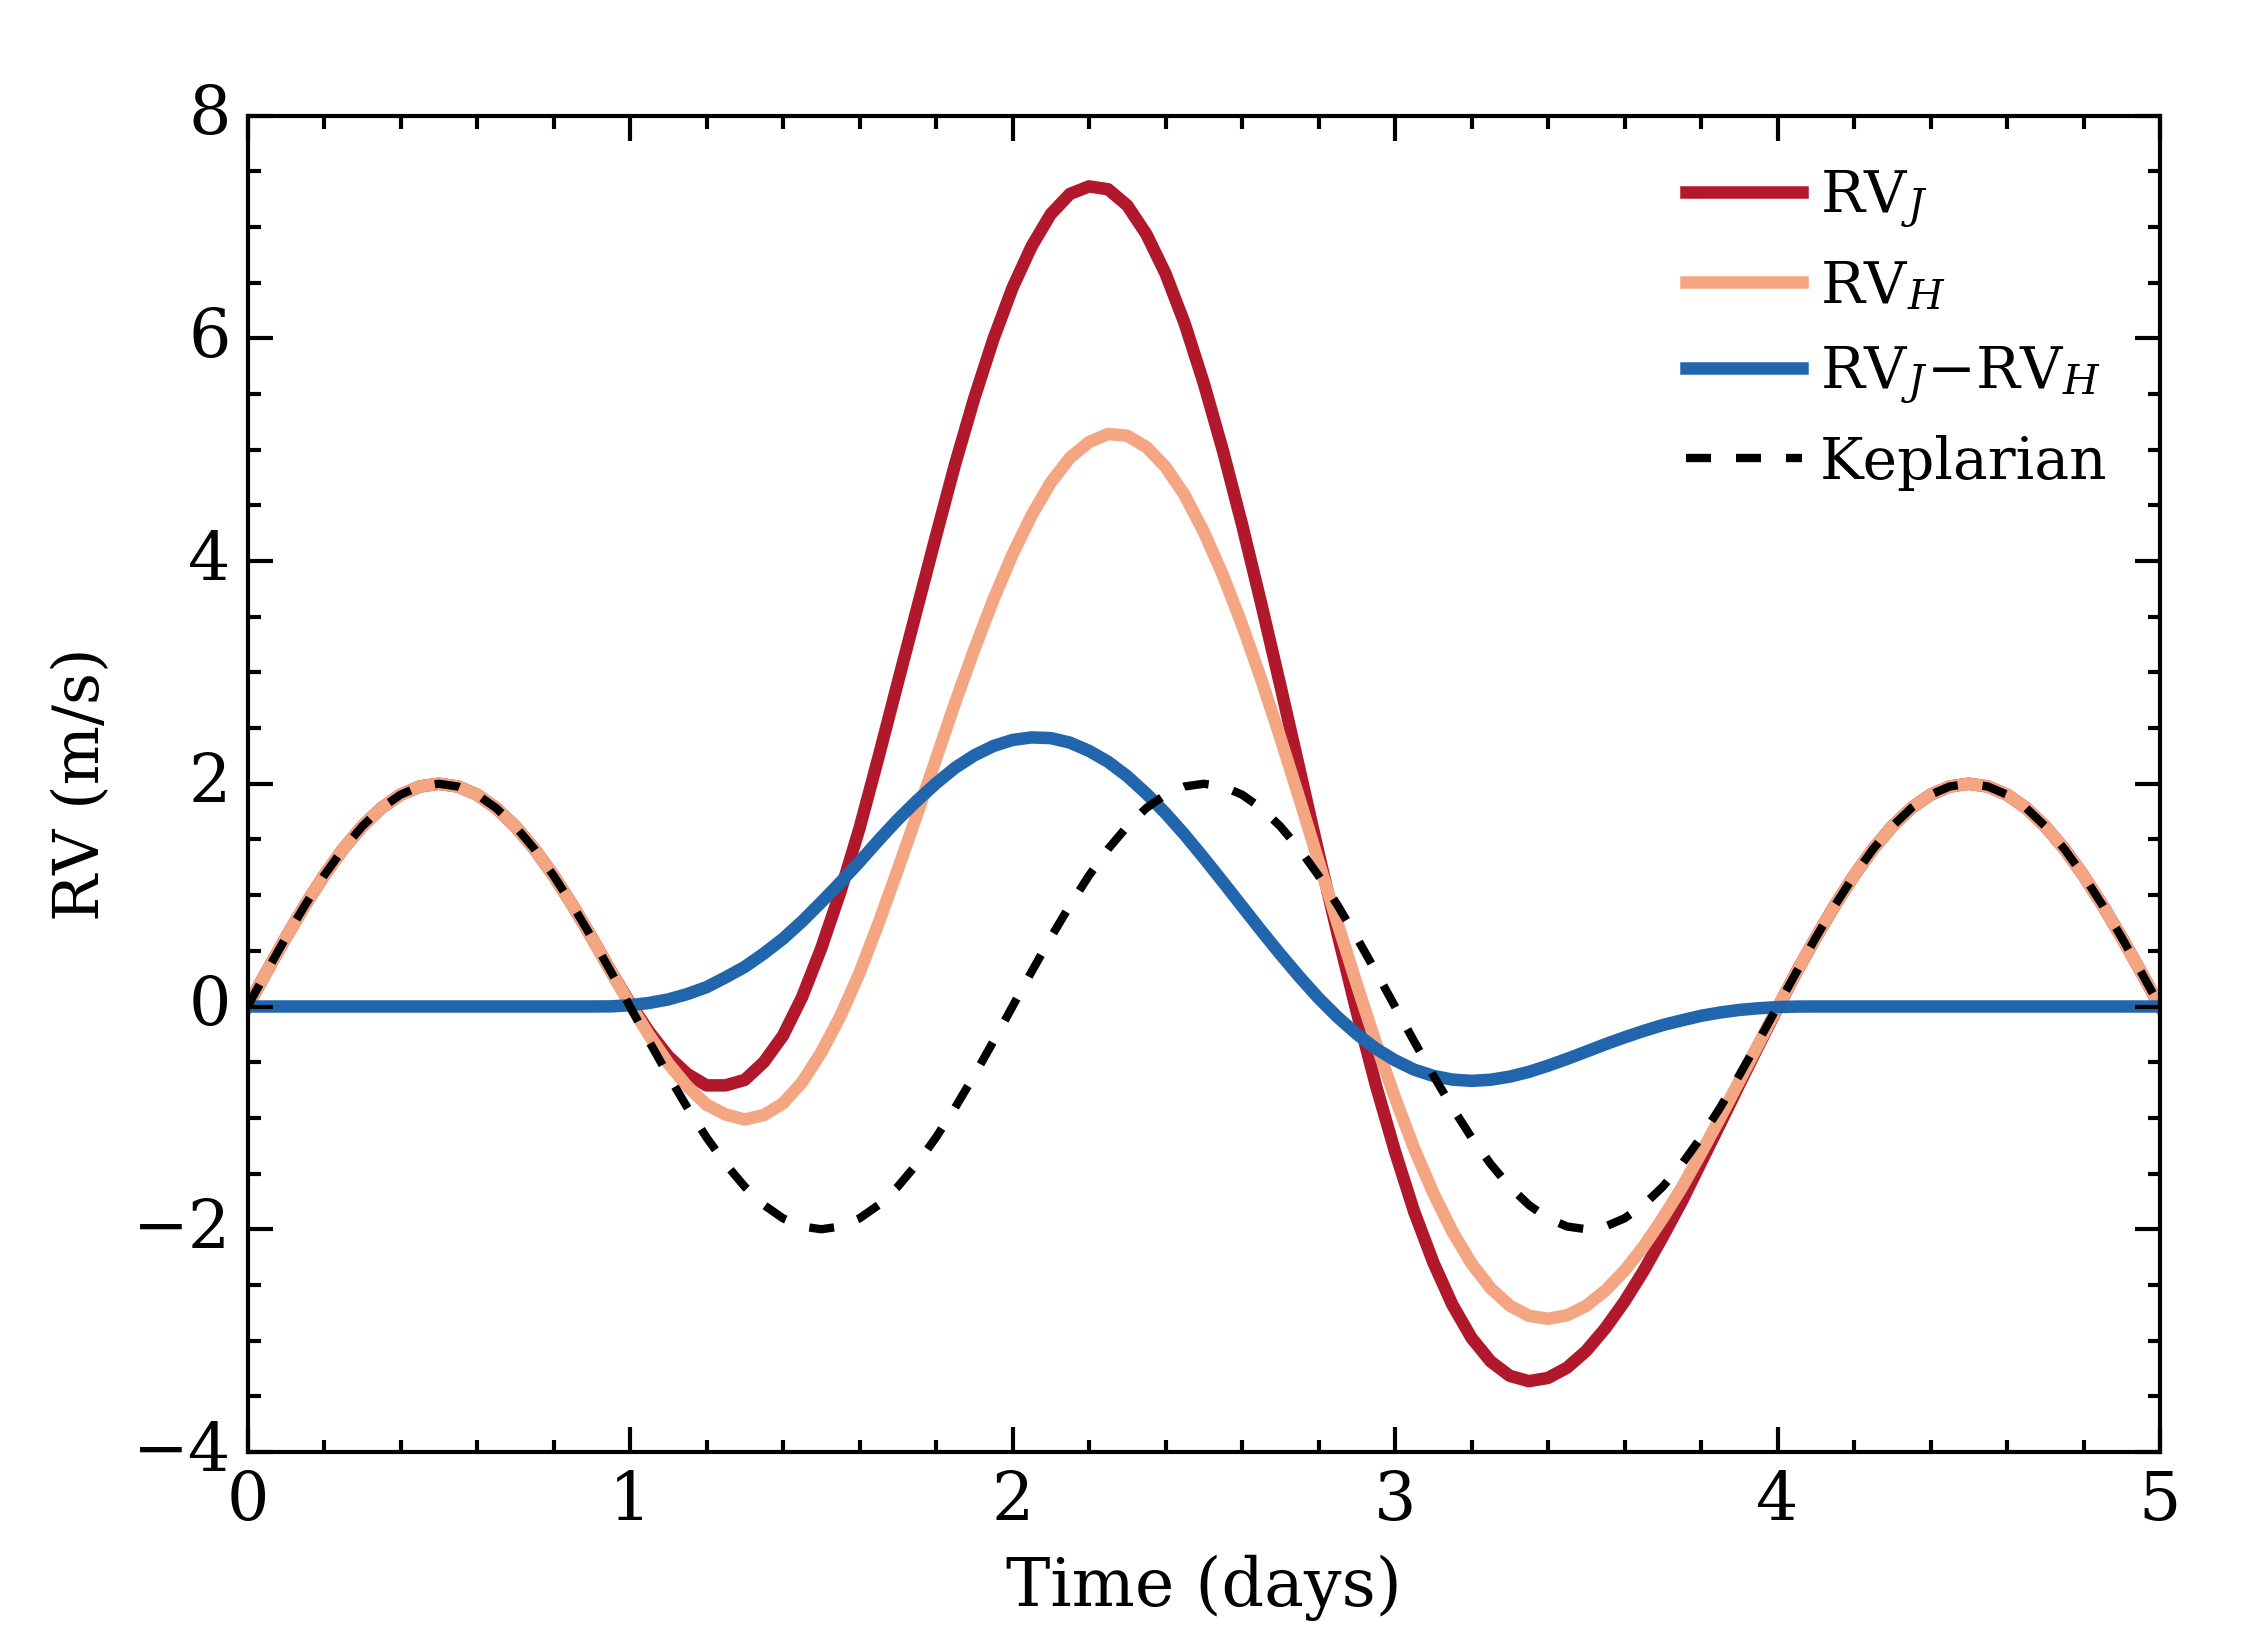
\includegraphics[scale=.6]{figures/rvjitterdiff.png}
\caption{Examples of noise-less radial velocity timeseries containing a single Keplarian 
signal (K$_1$; Eq.~\ref{eq:rvtot}) and a large equatorial spot computed with the 
\texttt{SOAP 2.0} code ($P_{\mathrm{rot}}=5$ days). 
The radial velocities contain the keplarian signal plus jitter from the flux 
and convective effects and are evaluated at the J band ($\lambda_1 \sim 1.2$ $\mu$m) and H band 
($\lambda_2 \sim 1.6$ $\mu$m). \label{fig:jitterdiff}}
\end{figure}

\subsection{Tomographic Modelling}
Akin to the Doppler-imaging technique discussed in Sect.~\ref{sect:spots}, the evolution of the 
Stokes I and V line profiles from polarimetry 
can be used to reconstruct surface maps of the stellar surface 
brightness and magnetic field strength with different orientations. The former maps are 
derived from the unpolarized spectra (Stokes I) and the latter from both 
the unpolarized and circularly polarized 
spectra (Stokes V) which are sensitive to the Zeeman signature (see Sect.~\ref{sect:zeeman}) 
indicative of the presence of 
magnetic fields. The map construction from timeseries of the Stokes I and V line profiles is 
known as \emph{tomographic modelling}. \\

Fig.~\ref{fig:stokes} 
shows examples of the normalized Stokes I and V line profiles over $\sim 4$ rotation 
cycles of the weak-line T-Tauri star LkCa 4 \parencite{donati14b}. The tomographic maps derived 
from those line profiles are also shown from one pole down to a latitude of $-30^{\circ}$. 
Knowledge of the location, contrast, and magnetic field strength on the stellar surface can 
be used to derive the contemporaneous radial velocity jitter. Indeed this procedure has be 
implemented and was used to uncover a very young hot Jupiter orbiting the T-Tauri star 
V830 Tau. In principle the Stokes Q and U profiles 
can also be used to improve magnetic field mapping but require much higher SNRs 
than Stokes V in order to detect their Zeeman signatures and are often neglected as a result. \\

\begin{figure}
\centering
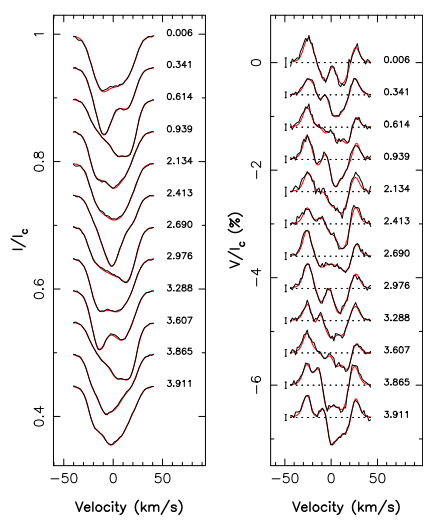
\includegraphics[scale=.5]{figures/stokes.png}
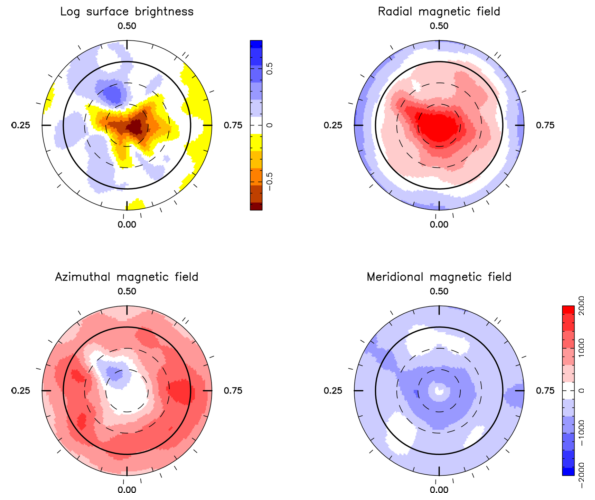
\includegraphics[scale=.5]{figures/tomographicmaps.png}
\caption{\emph{Top}: the observed (\emph{black}) and fit (\emph{red}) Stokes I (\emph{left}) 
and V (\emph{right}) normalized line profiles at 12 epochs over $\sim 4$ rotation cycles. 
\emph{Bottom}: tomographic maps of the stellar surface brightness and 3 spatial components of 
the magnetic field strength measured in Gauss. 
\parencite[Image credit:][]{donati14b} \label{fig:stokes}}
\end{figure}


\subsection{Concluding words on activity indicators}
With multiple ancillary timeseries which are sensitive to activity-related signals and not 
keplarian signals, if the jitter has any periodicity as we would expect if it was rotationally 
modulated, then it should be apparent in the frequency spectrum of each ancillary timeseries. 
Similarly any detectable keplarian periodicity should \emph{only} be apparent in the radial 
velocity timeseries itself. We can use these timescale arguments to help distinguish activity 
signals from planets. \\

This however leads to the complication that because any detectable keplarian periodicity and 
the stellar rotation periodicity may be significant in the frequency spectrum of the radial 
velocity timeseries, keplarian signals close to the stellar rotation period and/or its low-order 
harmonics will be confused. These confused periodic signals from planets are difficult to 
detect and indeed there is an intrinsic detection bias at the stellar rotation period 
\parencite{vanderburg16}. Based 
on the HZ separations and rotation period distribution for the various subclasses of M-dwarfs, 
\cite{newton16b} argued that M-dwarfs with spectral classes M4-M6 
($0.1 \lesssim M_s/$M$_{\odot} \lesssim 0.25$) 
represent the best possible candidates for finding habitable zone planets around cool stars.
 


\section{Models of Stellar Jitter} \label{sect:jittermodels}
There exists a number of analytical models of 
the radial velocity signal arising from certain sources of stellar jitter. The models which 
are discussed below only deal with the jitter arising from active regions. As a reminder, 
active regions on the surface of a star will i) break the homogeneity of the stellar disk causing 
an deficit of particularly Doppler-shifted photons depending on if the active region occults the 
approaching (blueshifted) or receding (redshifted) 
stellar limb (the flux effect), ii) will reduce the convective blueshift 
by suppressing the flow of hot granules to the surface and iii) will induce Zeeman broadening of 
the spectral lines in the presence of strong magnetic fields.

\subsection{FF$\mathbf{'}$ Method} \label{sect:ffprime}
The FF$'$ method is a popular model of the stellar radial velocity variations induced by the 
presence of dark or bright regions on its surface. The formalism, originally presented in \cite{aigrain12}, 
computes the radial velocity from the suppression of convective blueshift and the 
flux effect given 
an input timeseries of the fractional coverage of the visible stellar disk by active regions $F(t)$ 
which is derived from a photometric light curve $\Psi(t)$. 
As we shall see, the former jitter 
term only depends on the fractional coverage while the latter depends on 
$F$ and its first time derivative thus giving the method the name FF$'$. This method is commonly 
used to estimate the radial velocity jitter given a light curve from say \emph{Kepler} or \emph{TESS} 
but has also been used as a model of activity in radial velocity timeseries analysis 
\parencite[e.g.][]{haywood14}. \\

Given the light curve of a star whose radial velocity variations we are interested in 
computing, the approximate fractional coverage by active regions is 

\begin{equation}
F(t) = 1 - \frac{\Psi(t)}{\Psi_0} \label{eq:fractionalcoverage}
\end{equation}

\noindent where $\Psi_0$ is the assumed flux in the absence of active regions. 
The first time derivative 
of $F(t)$ is 

\begin{equation}
F^{'}(t) = -\frac{\Psi^{'}(t)}{\Psi_0}.
\end{equation}

\noindent These models neglect the effects of limb-darkening as the effect is argued to be small 
in \cite{aigrain12}. 
We also note that an accurate calculation of $F^{'}(t)$ from observations 
requires a smooth light curve model 
whose time derivative can be computed from simple methods such as finite differences. A Gaussian 
process can be of great use in computing such a model (see Sect.\ref{sect:covariance}). \\

\cite{aigrain12} write out the expected radial velocity signal for each source separately as a function of the stellar 
projected rotation velocity \vsini{} $=2 \pi R_s \sin{i_s} / P_{\mathrm{rot}}$, spot latitude $\delta$, 
angle between the spot normal and the 
line-of-sight $\beta(\phi,\delta,i_s)$, and the phase relative to the line-of-sight $\phi(t)$. 
The flux term written in terms of these geometric variables and in terms of observables is  

\begin{align}
\Delta \mathrm{RV_{flux}} (t) &= -F(t) v \sin{i_s} \cos{\delta} \sin{\phi(t)} \\
&= -F(t) F^{'}(t) \frac{R_s}{f}, \label{eq:flux}
\end{align}

\noindent where $f\approx (\Psi_0 - \Theta_{\mathrm{min}}) / \Psi_0$ and $\Theta_{\mathrm{min}}$ is the 
minimum observed flux. \\

The convective blueshift suppression term depends only on the fractional spot coverage and 
not its rate of evolution in time. Recall also that spots tend to be surrounded by magnetized areas 
(faculae/plages) 
which have a small temperature contrast with the surrounding photosphere and therefore have a small 
photometric effect but a significant spectroscopic effect. This is accounted for by a factor $\kappa$, 
typically $>1$ which amplifies the effect of $F(t)$ on the convective 
jitter term. $\kappa$ represents the ratio of 
the magnetized area to the spot surface. The amplitude of the convective signal 
is also dependent on the velocity difference between the spotted and unspotted photosphere $\delta V_c$. 
The convective term is then written as 

\begin{align}
\Delta \mathrm{RV_{conv}} (t) &= F(t) \delta V_c \kappa \cos{\beta(t)} \\
&= F^{2}(t) \delta V_c \frac{\kappa}{f}. \label{eq:conv}
\end{align}

\noindent The total radial velocity jitter signal from spots and their surrounding magnetized area is just the 
sum of Eqs.~\ref{eq:flux} and \ref{eq:conv} and \emph{can be estimated from a star's light curve 
without a priori knowledge of its rotation period.} Fig.~\ref{fig:ffprime} show the photometric 
signal and radial velocity jitter from a single spot on a star with $P_{\mathrm{rot}} = 5$ days, $\delta V_c = 200$ 
\mps{,} and $\kappa=10$. The dependence of $\Delta \mathrm{RV_{flux}}$ on $F^{'}(t)$ causes the change 
in slope of $\Delta \mathrm{RV_{tot}}$ during one occultation of a spot which, I should point out, 
looks an awful lot like the signal from a transiting planet. \\

\begin{figure}
\centering
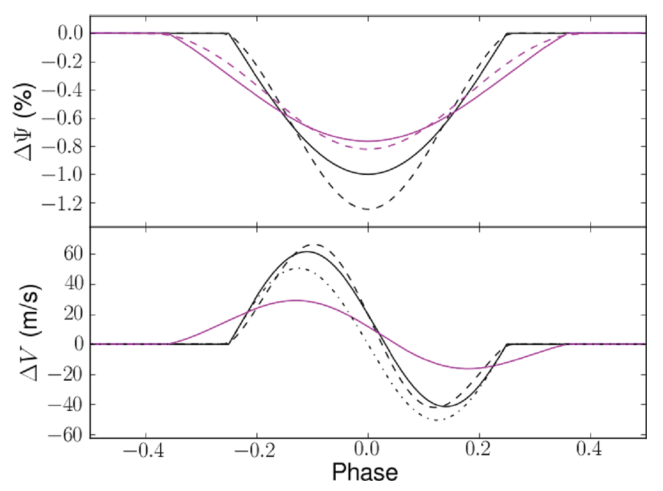
\includegraphics[scale=.5]{figures/ffprime.png}
\caption{Examples of simulated photometric (\emph{top}) and radial velocity (\emph{bottom}) signatures 
from a single spot with varied latitude and stellar inclination. \emph{Solid black line} depicts the signature 
from an equatorial spot with $i_s=90^{\circ}$. The \emph{cyan} 
is for a mid-latitude ($\delta=60^{\circ}$) spot with 
$i_s=70^{\circ}$. The \emph{dashed lines} are models of the same spots with the inclusion of a linear 
limb-darkening parameter $u=0.5$ \parencite{dorren87}. 
\parencite[Image credit:][]{aigrain12} \label{fig:ffprime}} 
\end{figure}

The star for which we have the greatest understanding of its noise properties is the Sun. 
\cite{dumusque15} used contemporaneous photometry and radial velocity measurements of the 
disk-integrated Sun to the observed Doppler shifts to predictions from the FF$'$ method 
using the photometry. The FF$'$ modelling of the radial velocity jitter from active regions 
was shown to perform ``efficiently'' but is still known to be unable to explain the full 
radial velocity variations from stellar noise \parencite[e.g.][]{aigrain12, haywood14}. 
Longer baseline observations of the Sun will allow the FF$'$ method to be scrutinized further 
\parencite{dumusque15}.

\subsection{\texttt{SOAP}} \label{sect:soap}
Software such as the Spot Oscillation and Planet code 
\parencite[\texttt{SOAP};][]{boisse12} 
can be used to compute the CCF resulting from the presence of active regions on a rotating star. 
The second version of this code \parencite[\texttt{SOAP 2.0};][]{dumusque14} 
is often used to model radial velocity variations and CCF distortions such as its 
full width at half maximum (see Sect.~\ref{sect:fwhm}) and its asymmetry (see Sect.~\ref{sect:bis}). 
\texttt{SOAP 2.0} is often favoured over its predecessor 
because it takes into account both the flux and convective 
effects whereas the original version of \texttt{SOAP} only modelled the former effect. \\

The basic methodology is illustrated in Fig.~\ref{fig:soapccf}. The stellar disk is discretized into a 
2D grid. Each grid cell has a Doppler shifted Gaussian CCF according to the projected rotation velocity 
(\vsini{)} at the cell's location. The intensity of each 
CCF is weighted by the adopted quadratic 
limb-darkening law \parencite{claret11} or by the temperature contrast of a dark spot or bright plage if 
the grid cell contains an active region. The code's output includes the photometric signal as well as 
radial velocity jitter, FWHM, and BIS timeseries 
resulting from the distortion of the CCF as either a spot or plage 
traverses the stellar disk over one rotation cycle. Therefore, the code does not take into account 
any evolution of an active regions size or contrast over time. The tunable parameters in the code are 
summarized in Table~\ref{table:soap}. \\


\begin{figure}
\centering
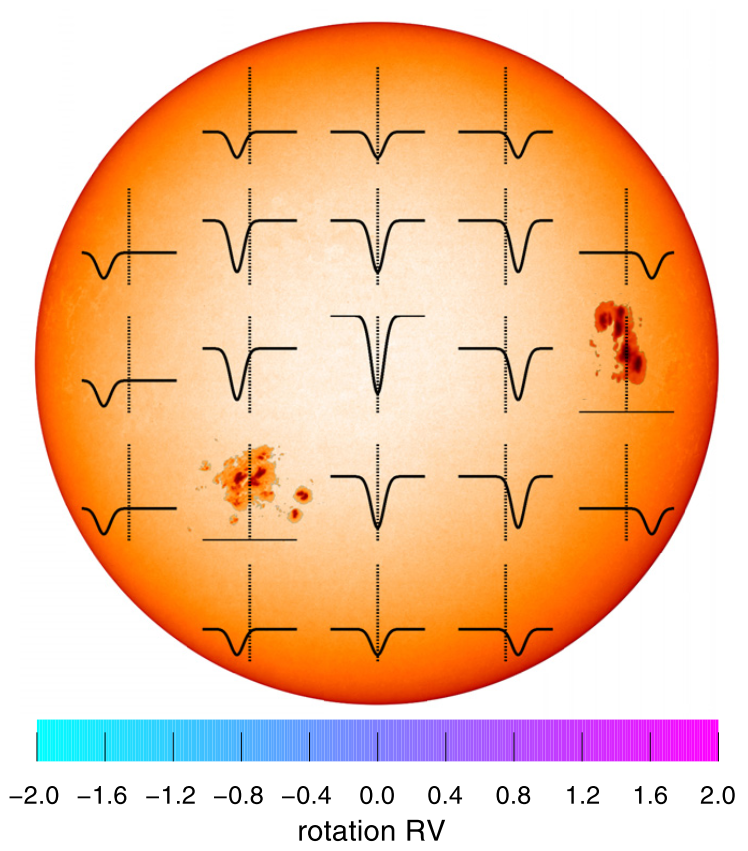
\includegraphics[scale=.3]{figures/soapccf.png}
\caption{A visual depiction of the treatment of the simulated CCF in the \texttt{SOAP 2.0} 
code for simulating the observable spectroscopic signatures of active regions. The final CCF 
at a single epoch is the integral of all the CCFs over the stellar disk. 
The projected radial velocity across 
the stellar disk is shown in the colour-bar in km s$^{-1}$. 
\parencite[Image credit:][]{dumusque14} \label{fig:soapccf}}
\end{figure}


\subsection{Zeeman Broadening} \label{sect:zeeman}
Spectral line profiles arising from regions embedded in a magnetic field, such as in active 
regions, are affected by the Zeeman effect. This is a quantum mechanical effect wherein 
the quantum number of the total angular momentum $J$ is split into $2J+1$ energy states 
with varying magnetic quantum numbers $M$ \parencite{reiners12c}. 
The energy level splitting gives rise to a characteristic splitting of the observed line 
profiles themselves (see Fig.~\ref{fig:zeeman}). \\

\begin{figure}
\centering
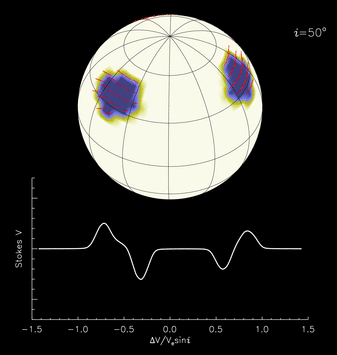
\includegraphics[scale=.5]{figures/zeeman.png}
\caption{An example of a star with small scale magnetic fields as seen on active late-type 
stars. The resulting spectral splitting in the Stokes V parameter (circular polarization 
measure) is due to the Zeeman effect of line splitting in the presence of a magnetic field. 
\parencite[Image credit:][]{kochukhov16} \label{fig:zeeman}}
\end{figure}

\cite{reiners13} model the impact of Zeeman broadening from active regions on the observed 
stellar radial velocity. They use polarized radiative transfer models to compute the  
Zeeman splitting with atomic and molecular Land\'{e} factors from the V band to K band. 
The Zeeman deformation to spectral lines 
depends on each split level's quantum numbers which are consolidated 
into the dimensionless Land\'{e} factor $g$ 
which depends on the absorbing species but is typically $\sim 1$ for atomic 
species and 
$\sim 0.6$ for the molecular species in M-dwarfs \parencite{shulyak10,reiners13}. \\

\cite{reiners13} 
then calculate the amplitude of the radial velocity jitter at a wavelength 
$\lambda$ from Zeeman broadening and 
derive the following scaling as a function of the magnetic field strength $B$:
%The amplitude of the Zeeman deformation will affect the measured radial velocities by 
%an amount according to 

\begin{equation}
\Delta \mathrm{RV}_{\mathrm{Zeeman}} = 300f \left(\frac{B}{1 \mathrm{kG}} \right)^2 
\left(\frac{\lambda}{1 \mu\mathrm{m}} \right)^a \mathrm{m} \hspace{2pt} \mathrm{s}^{-1}, 
\label{eq:zeeman}
\end{equation}

\noindent where $f$ is the active region's fractional area and the powerlaw index $a$ 
was shown to vary from $\sim 2$ for hot Sun-like stars to $<2$ for cooler stars. 
\cite{reiners13} performed this calculation for a typical Sun-like star ($T_{\mathrm{eff}}=5750$ K), 
early M-dwarf ($T_{\mathrm{eff}}=3700$ K), and late M-dwarf ($T_{\mathrm{eff}}=2800$ K). The 
exact value of $a$ was shown to depend primarily on the magnetic field strength (treated as a 
free parameter) and $T_{\mathrm{eff}}$. \\

A first-order estimate of the 
contribution to the radial velocity jitter from Zeeman broadening can be made using 
Eq.~\ref{eq:zeeman} for stars whose rotation periods have been measured from 
photometric variability. Recall that one can derive the fractional coverage by magnetized 
regions $f$ from a star's light curve ($f=F$; Eq.~\ref{eq:fractionalcoverage}). Empirical 
correlations between magnetic field strength, activity levels, and stellar rotation have 
been found (see Fig.~\ref{fig:Bfields}). We can use these correlations to draw an approximate 
value of $B$, given $P_{\mathrm{rot}}$ as a starting point, and estimate the corresponding 
radial velocity jitter from Zeeman broadening. \cite{reiners13} found that 
``the amplitude of the radial velocity signal caused by the Zeeman effect alone can be comparable to that 
caused by temperature contrast; a spot magnetic field of $\sim 1000$ G can produce a similar 
radial velocity amplitude as a spot temperature contrast of $\sim 1000$ K.'' \\

\begin{figure}
\centering
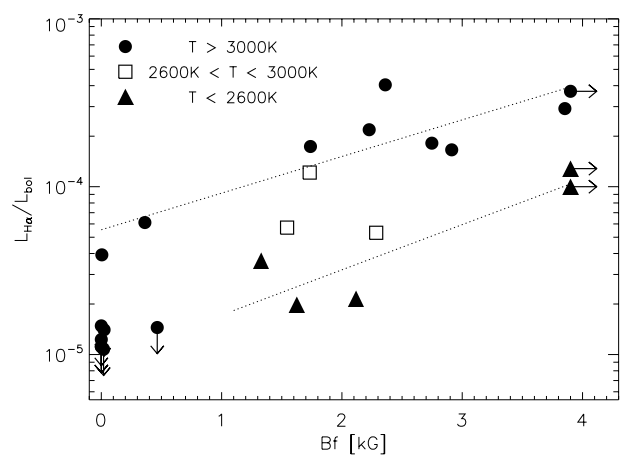
\includegraphics[scale=.4]{figures/LHalpha_B.png}
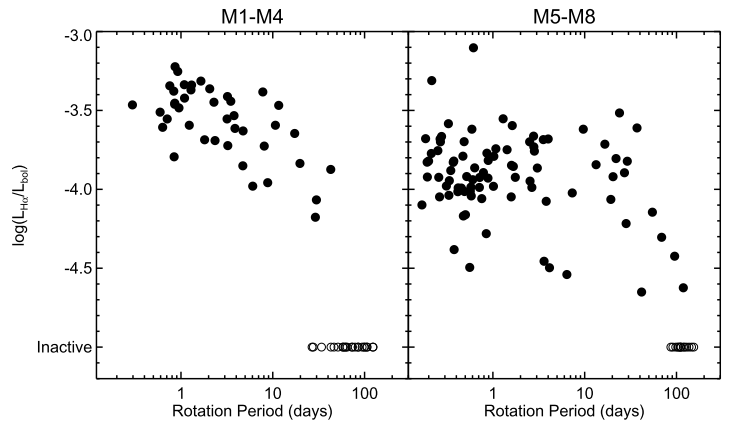
\includegraphics[scale=.4]{figures/LHalpha_Prot.png}
\caption{\emph{Top}: the empirical correlation between the effective magnetic field strength 
($|\mathbf{B}| \times$ the filling factor $f$) and the relative H$\alpha$ luminosity for 
stars in various effective temperature ranges \parencite[Image credit:][]{reiners07}. 
\emph{Bottom}: the empirical correlation 
between the stellar rotation period and relative H$\alpha$ luminosity for early-to-mid and 
mid-to-late M-dwarfs \parencite[Image credit:][]{west15} \label{fig:Bfields}}
\end{figure}

It is also noted that typical values of $a>0$, the positive scaling of 
$\Delta \mathrm{RV}_{\mathrm{Zeeman}}$ with 
$a$ implies that the effect of Zeeman broadening grows with increasing wavelength unlike the 
jitter arising 
from temperature contrast in active regions alone. In fact, in very active late-type stars 
the increase in Zeeman jitter with $\lambda$ may dominate over the decrease in temperature 
contrast related jitter at longer wavelengths \parencite{reiners13}. As was previously alluded, 
the amplitude of the radial velocity jitter may or may not increase towards near-IR wavelengths 
from the optical regime. This is especially true for 
active stars in which Zeeman broadening can have a 
significant contribution to the total jitter.

\section{Point-form Thesis: Stellar Jitter}
\begin{itemize}
\renewcommand\labelitemi{--}
\item~\ref{sect:jitter} \textbf{Sources of Stellar Jitter}: there is a plethora of physical 
processes ongoing in and above a star's photosphere which result in unwanted radial velocity 
signals that can mask or mimic planetary signals. 
See Table~\ref{table:jitter} for a summary of their approximate timescales and amplitudes. 
\item~\ref{sect:diagnostics} \textbf{Activity Indicators}: photometric, 
spectroscopic, and polarmetric 
timeseries can be used to inform models of the radial velocity jitter thus helping to facilitate 
the detection of small amplitude planetary signals. 
\item~\ref{sect:jittermodels} \textbf{Models of Stellar Jitter}: there are tools to model the 
radial velocity jitter from the fractional coverage of the visible stellar disk by 
magnetized regions such as cool spots, hot faculae, and hot chromospheric plages.
\end{itemize}
